\subsubsection{Combinations of Fungal Species}
The distribution of fungi in the nature is diverse and wide, and there are often hundreds of microorganisms in one square meter of natural land~\cite{land}. In order to simplify the study on the topic that \textbf{combinations of fungal species likely to persist in different environment conditions}, we only analyze and predict the growth and decomposition ability of two fungi in combination.
\par
Since the known information is not sufficient and the internal relationship of fungal species combinations in different environments has a degree of uncertainty, we use \textbf{Gray Prediction Model}~\cite{gray} and time series data based on the \textbf{Decomposition Models} in \textit{Model~4.1} and \textit{Model~4.2} to analyze and predict the living situation of the fungal species combination and the change trend of decomposition ability.
\par
Mark the known group of time series data as follows.
$$X^0 = (x^0(1),\ x^0(2),\ x^0(3),\ \ldots,\ x^0(n))$$
\par
To ensure the stability of the data, we perform \textbf{Accumulated Generating Operation} (AGO)~\cite{gray} on the data. The AGO process would be executed multiple times until the time series data is stable enough, and we get the following time series data.
$$X^1 = (\sum^1_{i=1}x^0(i),\ \sum^2_{i=1}x^0(i),\ \ldots,\ \sum^n_{i=1}x^0(i))$$
\par
The time series $X^1$ is then fitted by a first-order differential equation given by \textit{Eq.~(\ref{15eq})}
\begin{equation}
  \label{15eq}
  \frac{dx^1}{dt} = ax^1 = b
\end{equation}
where the parameters $a$ and $b$ are the development coefficient and control variable.
\par
According to the \textbf{whitening gray derivatives} of discrete data points, the following equation is obtained.
\begin{equation}
  \frac{dX^1(t)}{dt} = x^1(k) - x^1(k-1) = x^0(k)
\end{equation}
\par
A new variable $z^1(k)$, which is known as the whitening value of $x^1(k)$, is defined by the following equation.
\begin{equation}
  z^1(k) = 0.5x^1(k) + 0.5x^1(k-1)
\end{equation}
\par
Then we use \textbf{the least square method} to calculate the parameters.
\begin{equation}
  \hat{\delta} = (B^\top B)^{-1}B^\top Y
\end{equation}
where
$$\hat{\delta} = [\hat{a},\ \hat{b}]^\top,\ B=\left[ \begin{array}{cc}
      -z^1(2) & 1      \\
      -z^1(3) & 1      \\
      \vdots  & \vdots \\
      -z^1(n) & 1
    \end{array}
    \right],\ Y=\left[ \begin{array}{c}
      x^0(2) \\
      x^0(3) \\
      \vdots \\
      x^0(n)
    \end{array}
    \right]$$
\par
Finally, use \textbf{inverse AGO} and get the predicted value $x^2(k+1)$ as follows.
$$\hat{x}^2(k+1) = \hat{x}^1(k+1) - \hat{x}^1(k) = (1-e^a)(x^1(1) - \frac{b}{a})e^{-at},\ k = 1,\ 2,\ \ldots,\ n$$
\par
When new data are added, the parameters $a$ and $b$ in the Gray Prediction Model would be \textbf{updated} to ensure the accuracy of prediction.
\par
Due to the large differences in the suitable environment among the five fungi, we divide the five fungi into four combinations, including $F_A\ \&\ F_B$, $F_B\ \&\ F_C$, $F_C\ \&\ F_D$, and $F_D\ \&\ F_E$, based on the conclusion of \textit{Table~\ref{correspondingoptimalenvironment}} for analysis and prediction.
\par
Take combination $F_A\ \&\ F_B$ as an example. Calculate the time series data of the decomposition rate for the previous $122$ days using the data in \textit{Eq.~(\ref{sixtheq})}, \textit{Eq.~(\ref{ninetheq})}, and \textit{Table~\ref{decompositionrates}}, and mark it as follows.
$$X^0_{A\&B} = (x^0_{A\&B}(1),\ x^0_{A\&B}(2),\ \ldots,\ x^0_{a\&B}(122))$$
\par
Then the time series data is substituted into Gray Prediction Model, and the prediction data is calculated as follows.
$$X^2_{A\&B}=(x^2_{A\&B}(123),\ x^2_{A\&B}(124),\ \ldots,\ x^2_{A\&B}(200))$$
\par
Draw the decomposition rate of fungal species combination $F_A\ \&\ F_B$ in five climates, including arid, semi-arid, temperate, arboreal, and tropical rain forests, as shown in the figure below.
\begin{figure}[H]
  \centering
  \label{decompositioninfiveclimates}
  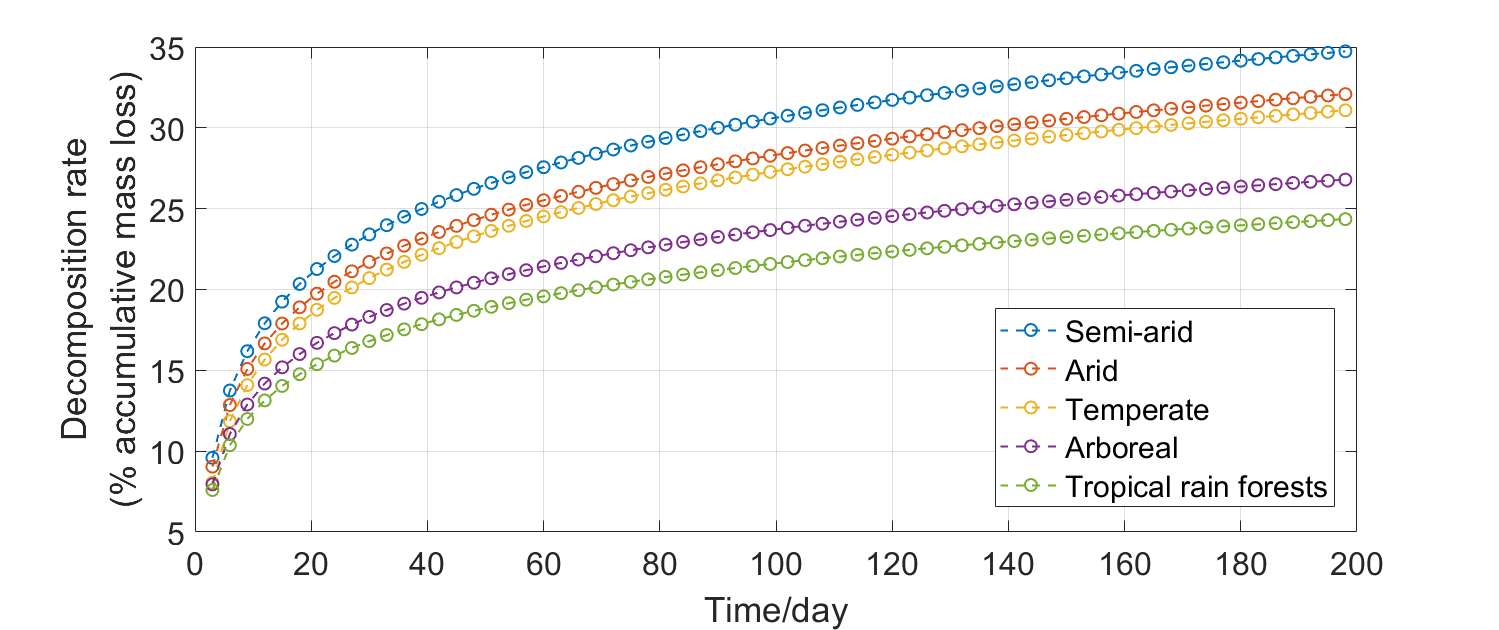
\includegraphics[width=\textwidth]{figures/A&B.png}
  \caption{Decomposition rate of fungal species combination $F_A\ \&\ F_B$ in five climates.}
\end{figure}
Combination $F_A\ \&\ F_B$ is most suitable for the decomposition of lignin or cellulose in semi-arid climate. From the prediction result, the cumulative decomposition rate after $200$ days can reach $34.7\%$.
\par
In the same way, the time series data of the other three fungal species combinations, $F_B\ \&\ F_C$, $F_C \&\ F_D$ and $F_D \&\ F_E$, are calculated as follows.
\begin{equation*}
  \begin{cases}
    X^0_{B\&C} = (x^0_{B\&C}(1),\ x^0_{B\&C}(2),\ \ldots,\ x^0_{B\&C}(122)) \\ \\
    X^0_{C\&D} = (x^0_{C\&D}(1),\ x^0_{C\&D}(2),\ \ldots,\ x^0_{C\&D}(122)) \\ \\
    X^0_{D\&E} = (x^0_{D\&E}(1),\ x^0_{D\&E}(2),\ \ldots,\ x^0_{D\&E}(122))
  \end{cases}
\end{equation*}
\par
Substituting Gray Prediction Model to obtain the following decomposition rate prediction curves in different climates in turn.
\par
\begin{figure}[H]
  \centering
  \subfigure[$F_B\ \&\ F_C$]{
    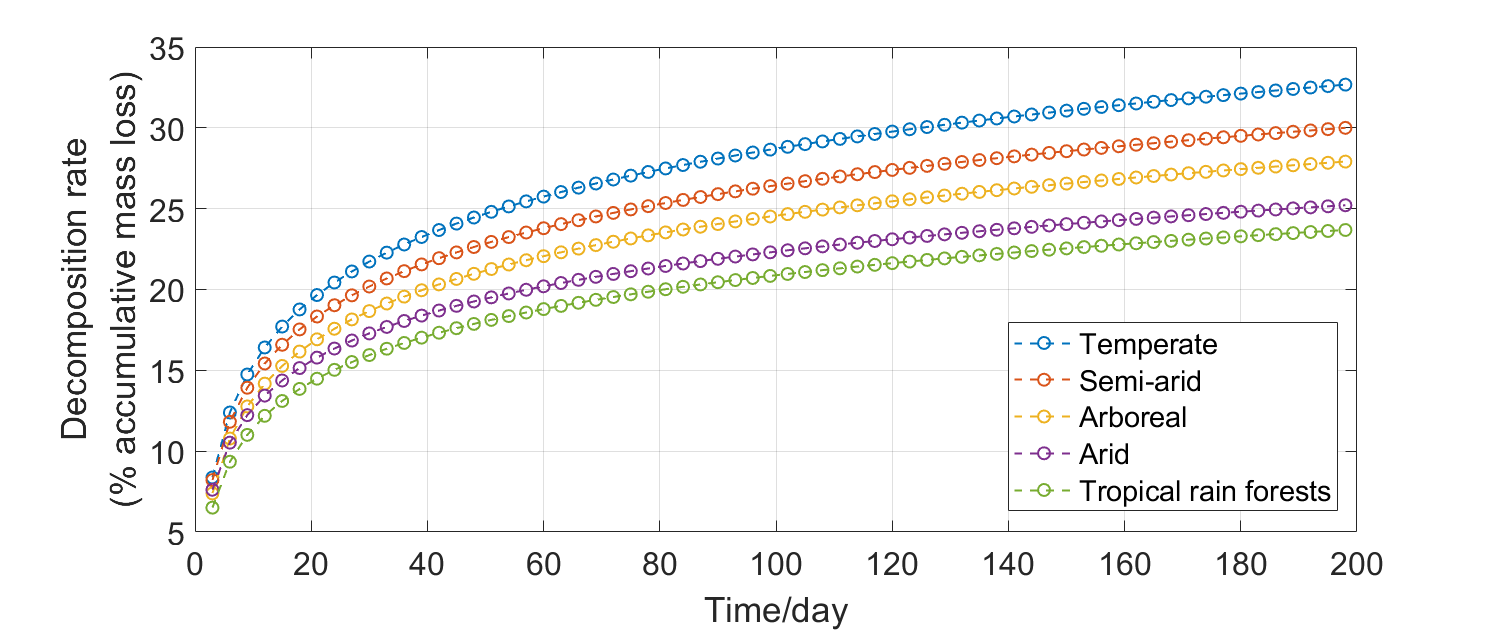
\includegraphics[width=0.95\textwidth]{figures/B&C.png}
  }
\end{figure}
\begin{figure}[H]
  \centering
  \subfigure[$F_C\ \&\ F_D$]{
    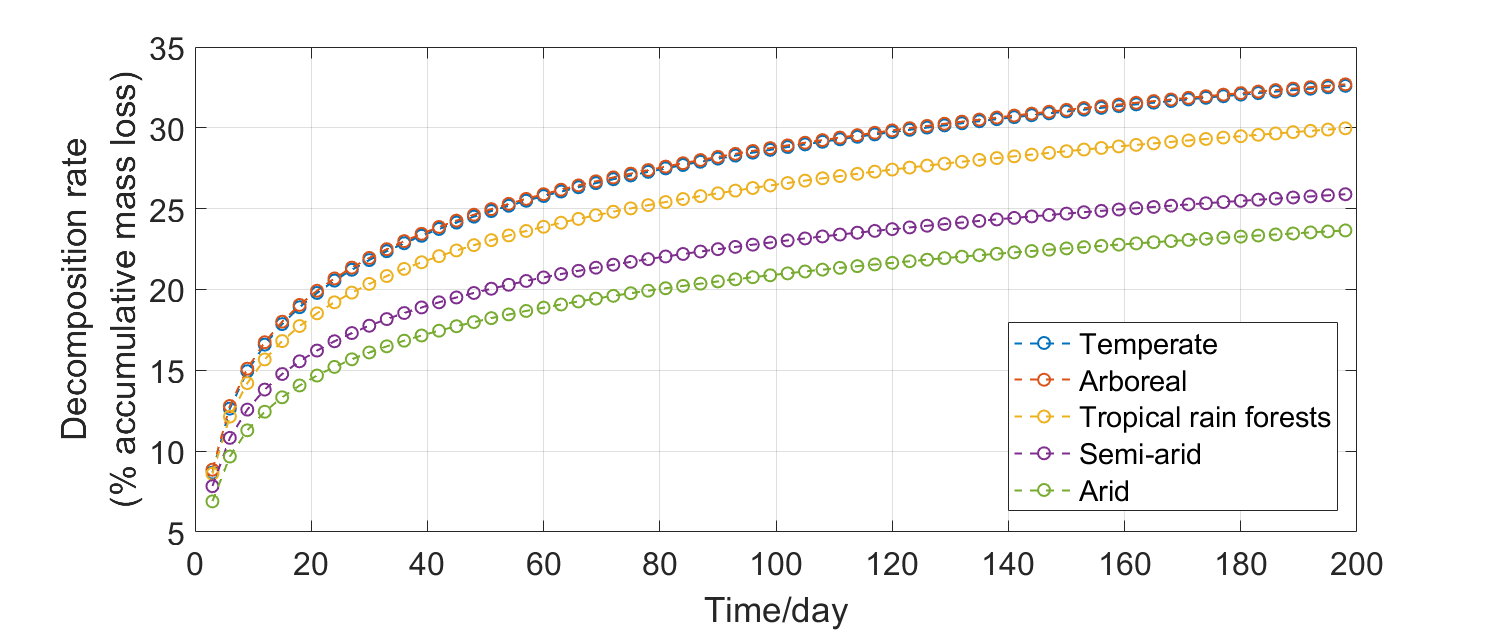
\includegraphics[width=0.95\textwidth]{figures/C&D.png}
  }
\end{figure}
\begin{figure}[H]
  \centering
  \subfigure[$F_D\ \&\ F_E$]{
    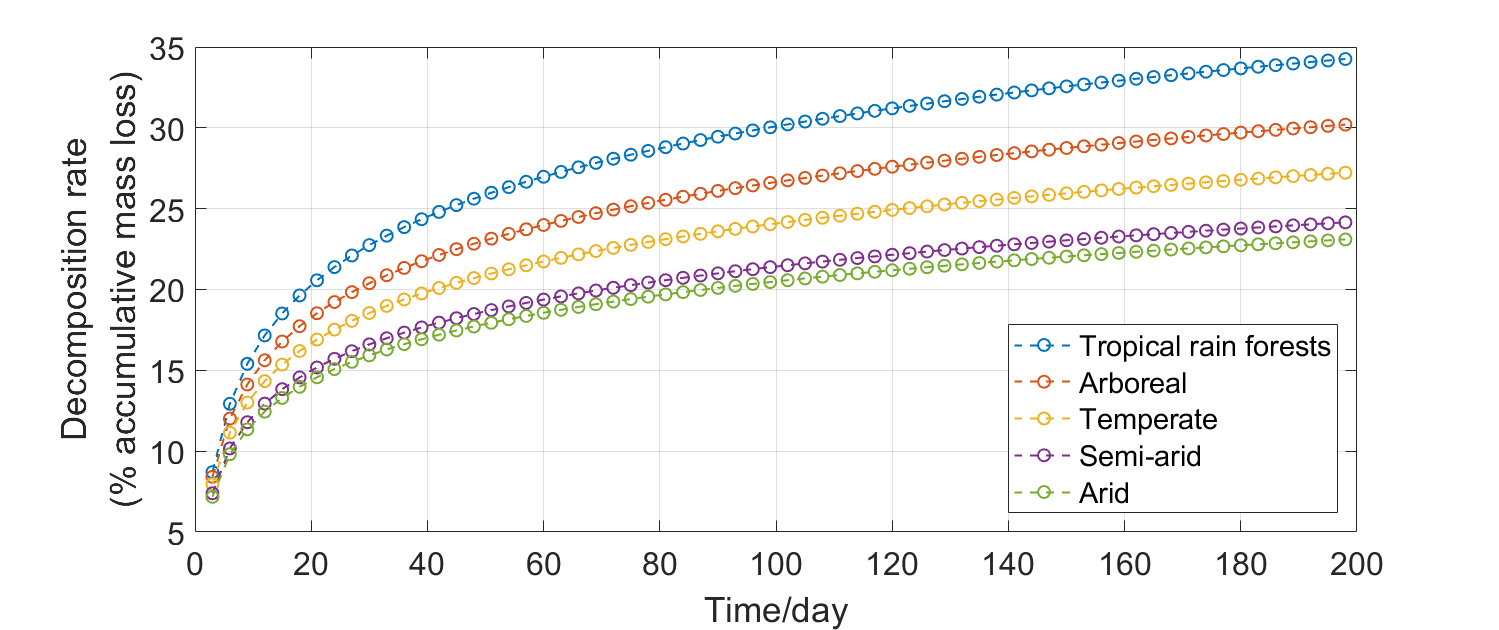
\includegraphics[width=0.95\textwidth]{figures/D&E.png}
  }
  \caption{Decomposition rate of fungal species combinations in five climates.}
\end{figure}
\par
The optimal environment and the predicted decomposition rate after $200$ days under different combinations of fungal species are summarized in the following table.
\begin{table}[H]
  \centering
  \caption{Summary of optimal environment and predicted decomposition rate.}
  \label{summaryofenvironmentandprediction}
  \begin{tabular*}{\hsize}{@{\extracolsep{\fill}}ccc}
    \toprule
    Combinations & Optimal Environment & Decomposition Rate Predicted Value \\
    \midrule
    $F_A\&F_B$ & Semi-arid & $34.7\%$ \\
    $F_B\&F_C$ & Temperate & $32.8\%$ \\
    $F_C\&F_D$ & Temperate / Arboreal & $32.7\%$ \\
    $F_D\&F_E$ & Tropical rain forests & $34.3\%$ \\
    \bottomrule
  \end{tabular*}
\end{table}
According to the above table, we find that the combination of $F_A\ \&\ F_B$ has the highest decomposition rate in semi-arid region, which is $34.7\%$, and the decomposition rates of other species combinations in their optimal environment are also relatively high, which are all above $32\%$.